\columnbreak
\section{Inselsysteme}

\begin{itemize}
    \item Einsatz in abgelegenen Regionen (z.B. Berghütten, Inseln)
    \item Typen
        \begin{itemize}
            \item PV-Inselsysteme
            \item PV-Pumpensysteme
            \item Mikronetze
        \end{itemize}
    \item Dimensionierung:
    \begin{itemize}
        \item Ermittlung Strombedarf
        \item Auslegung Batteriespeicher (Autonomiezeit, Kapazität)
        \item Dimensionierung Solargenerator auf schwächsten Monat
    \end{itemize}
\end{itemize}
%\begin{comment}
\subsubsection{Aufbau Inselsysteme}

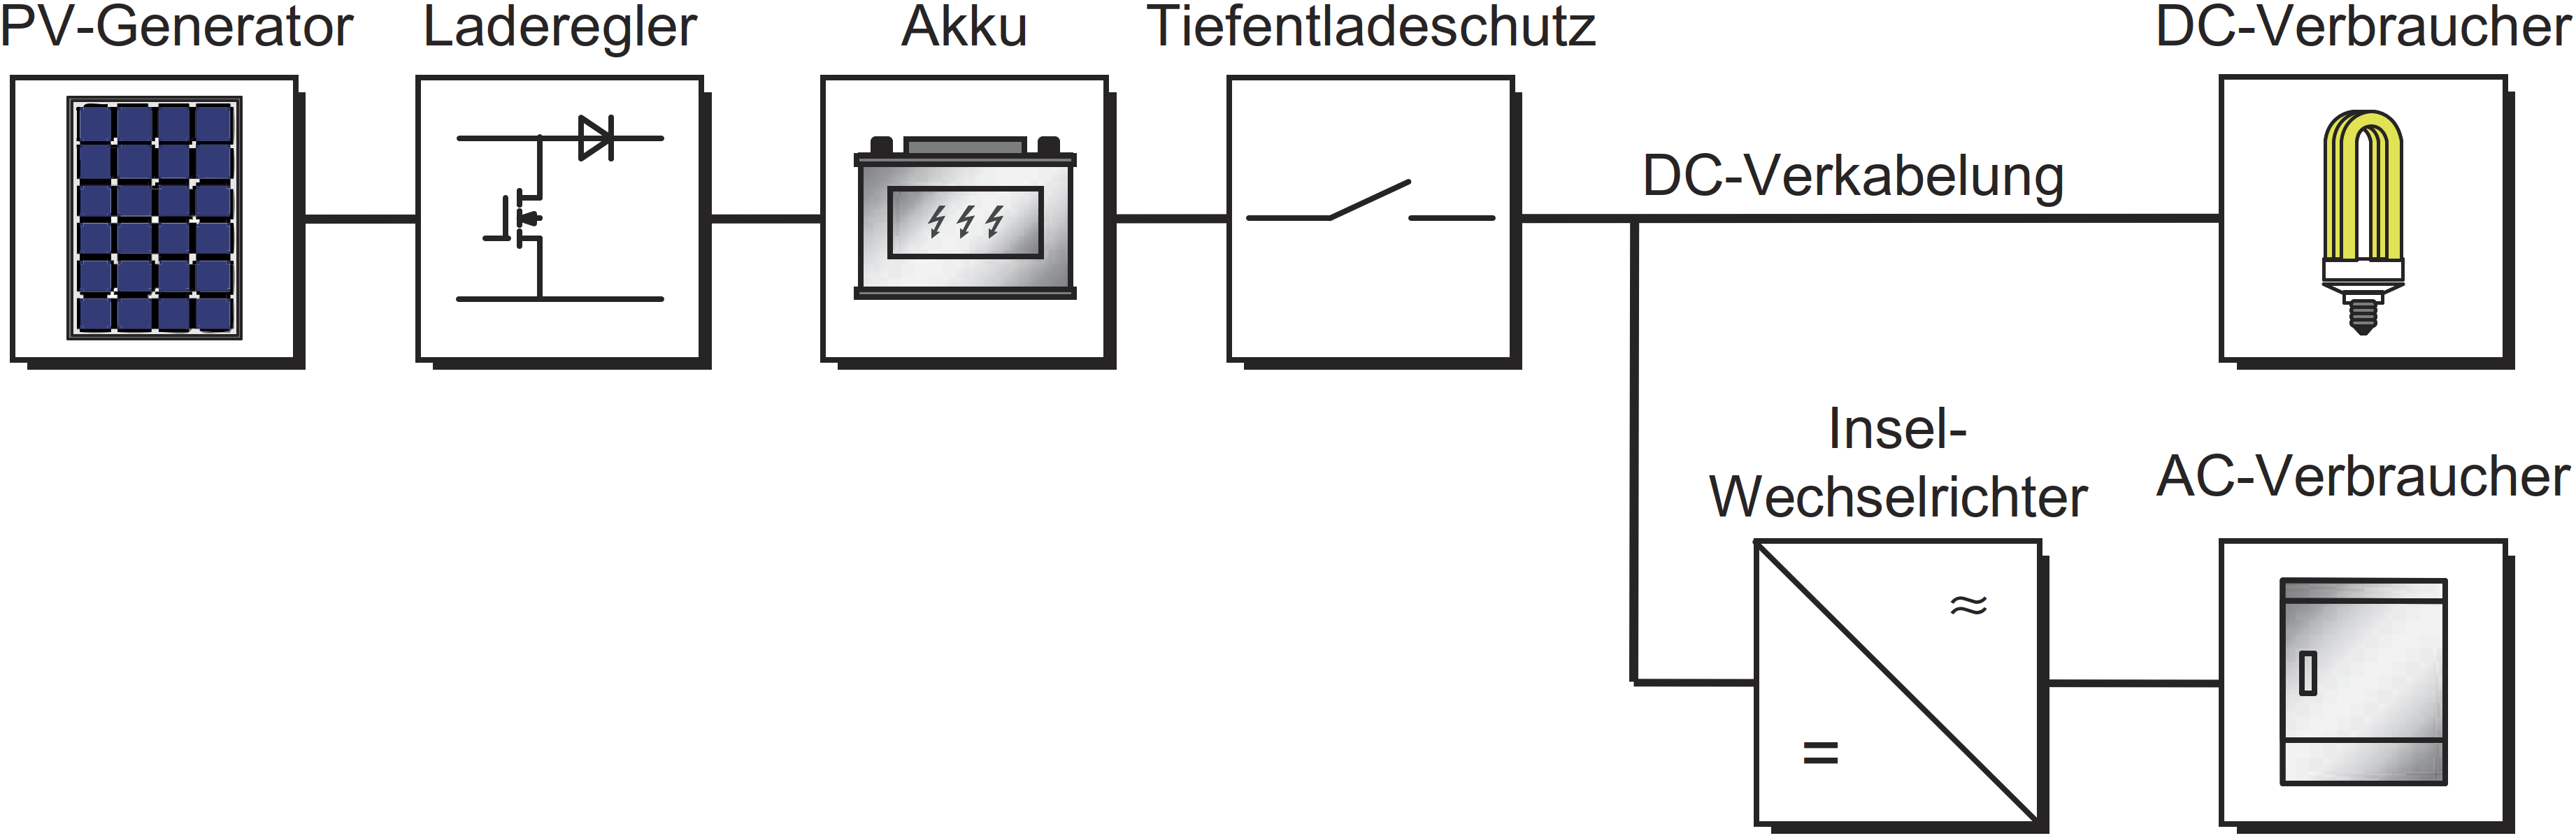
\includegraphics[width=0.98\linewidth]{images/Inselsysteme.png}
%\end{comment}

\subsection{Dimmensionierung}

\subsubsection{Ermittlung Stromverbrauch}

\begin{itemize}
    \item Nutzungsprofil: Saison/Monate, Anzahl Tage (z.B. Wochenendhaus)
    \item Bedarfstabelle täglicher Verbrauch
\end{itemize}

\subsubsection{Dimmensionierung Batteriespeicher}

\begin{itemize}
    \item Wahl Batterietyp: z.B. Blei (seltene Nutzung / wenige Zyklen) oder Lithium-Ionen (tägliche Nutzung)
    \item Gewünschte Autonomiezeit in Tagen (gewünschte Versorgungssicherheit)
    \item Maximale Last
\end{itemize}

\vspace{0.15cm}

$
\boxed{
C_{\mathrm{N}} = \frac{W \cdot N_{\mathrm{A}}}{U_{\mathrm{N}} \cdot \eta_{\mathrm{S}} \cdot DOD \cdot SOH_{\mathrm{min}}}
}
\quad \text{oder} \quad
\boxed{
C_{\mathrm{N}} = \frac{P_{\mathrm{max}} \cdot t_{\mathrm{disc}}}{U_{\mathrm{N}}}
}
$

$\boxed{\text{C-Rate} = \frac{P}{W}}$
\quad
$\boxed{R_{\mathrm{eig}} = \frac{W_{\mathrm{eig}}}{W_{\mathrm{PV,AC}}}}$
\quad
$\boxed{R_{\mathrm{Autarkie}} = \frac{W_{\mathrm{eig}}}{W_{\mathrm{ges}}}}$
\quad
$\boxed{R_{\mathrm{PV}} = \frac{W_{\mathrm{PV,AC}}}{W_{\mathrm{ges}}}}$


\renewcommand{\arraystretch}{1.2}
\begin{tabular}{@{} l p{6.5cm} l @{}}
    $[C_{\mathrm{N}}]$           & Nennkapazität der Batterie \dotfill                                  & $\mathrm{Ah}$ \\
    $[W]$                        & Elektrischer Energiebedarf pro Tag \dotfill                          & $\mathrm{Wh/d}$ \\
    $[N_{\mathrm{A}}]$           & Autonomiezeit (Tage ohne Nachladung) \dotfill                        & $\mathrm{d}$ \\
    $[P_{\mathrm{PV}}]$          & Nennleistung des PV-Generators \dotfill                              & $\mathrm{W_p}$ \\
    $[H_{i,\mathrm{gen}}]$       & Monatsmittlere Tagesstrahlungssumme auf geneigte Fläche \dotfill     & $\frac{\mathrm{Wh}}{\mathrm{31 \cdot d \cdot m^2}}$ \\
    $[\eta_{\mathrm{S}}]$        & Wirkungsgrad der Ausspeicherung \dotfill                             & $-$ \\
    $[DOD]$                      & Entladetiefe (Depth of Discharge) \dotfill                           & $-$ \\
    $[SOH_{\mathrm{min}}]$       & Minimaler State of Health / Gesundheitszustand \dotfill              & $-$ \\
    $[P_{\mathrm{max}}]$         & Maximale gleichzeitige Verbraucherleistung \dotfill                  & $\mathrm{W}$ \\
    $[k]$                        & Sicherheitsfaktor \dotfill                                           & $-$ \\
    $[\eta_{\mathrm{Sys}}]$      & Systemwirkungsgrad \dotfill                                          & $-$ \\
    $[U_{\mathrm{N}}]$           & Systemspannung \dotfill                                              & $\mathrm{V}$ \\
    $[SOC]$                      & Ladezustand in \% \dotfill                                           & \% \\
    $[\text{C-Rate}]$            & Entladerate ($P/W$) \dotfill                                         & $\mathrm{h^{-1}}$ \\
    $[t_{\mathrm{disc}}]$        & Minimale Entladezeit \dotfill                                       & $\mathrm{h}$ \\
    $[R_{\mathrm{eig}}]$         & Eigenverbrauchsquote \dotfill                                        & \% \\
    $[R_{\mathrm{Autarkie}}]$    & Autarkiegrad \dotfill                                                & \% \\
    $[R_{\mathrm{PV}}]$          & PV-Ertragsverhältnis \dotfill                                       & \% \\
\end{tabular}


\subsubsection{Faustregeln für Kapazitätsauslegung}
Zwischen 100\% - 150\% der PV-Leistung\\
oder zwischen 90\% - 120\% des Stromverbrauches\\
Es sollte ein gerundeter Wert gewählt werden (Reale Welt und so)\\
Autarkie und Eigenverbrauch werden bei Dimensionierung grösser als eines Tagesspeichers nicht grösser.\\
Die C-Rate soll mind. 0.3kW pro kWh Ladeleistung betragen.\\
\subsubsection{Dimmensionierung Solargenerator}

\begin{itemize}
    \item Wird auf den Strahlungsschwächsten Monat ausgelegt!
\end{itemize}

\vspace{0.15cm}

$\boxed{P_{\text{PV}}= \frac{W \cdot k \cdot 1'000 \frac{\textbf{W}}{\textbf{m$^2$}}}{H_{i,\text{gen}} \cdot \eta_{\text{Sys}}}}$



\subsubsection{Mikronetze}

\begin{itemize}
    \item Meist als Hybridsystem mit AC-Kopplung der Erzeuger und Verbraucher
    \item Speicherdimensionierung sehr individuell je nach Energieerzeugung, Verbrauchern etc.
    \item Bei größeren Systemen häufig Hybridbatterie als »Leistungsbatterie« (z.B. Lithium) und »Energiebatterie« (z.B. Redox-Flow)
\end{itemize}

\subsection{Autarkiegrad}
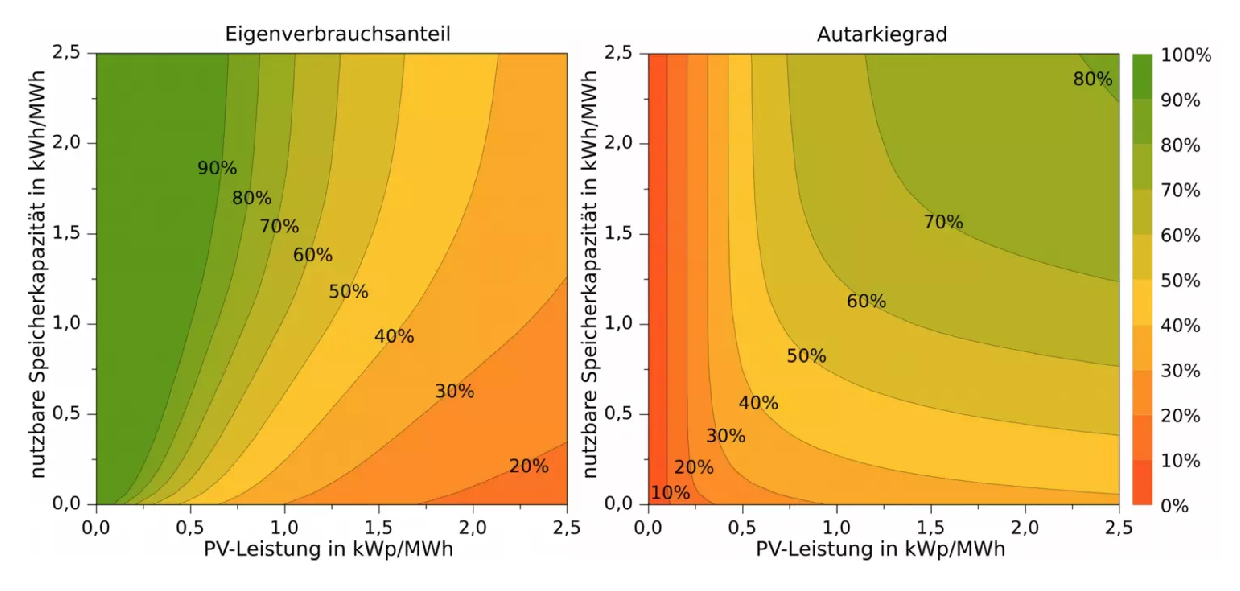
\includegraphics[width=0.98\linewidth]{images/Autarkiegrad.pdf}\\
\begin{itemize}
    \item Immer Systemeffizienz und Eigenverbrauchquote bei Auslegung beachten.
    \item Systemeffizienz wird beinflusst durch:
    \item Umwandlungswirkungsgrade (AC-DC)
    \item DC - Verluste
    \item Standby-Verbrauch
\end{itemize}